\documentclass{article}
\usepackage{iclr2027_conference,times}
\input{math_commands.tex}

\usepackage{hyperref}
\usepackage{url}
\usepackage{booktabs}
\usepackage{amsmath,amssymb}
\usepackage{amsthm}
\usepackage{graphicx}
\usepackage{xcolor}
\usepackage{tikz}
\usetikzlibrary{arrows.meta,positioning,shapes.geometric}
\newtheorem{proposition}{Proposition}
\definecolor{repairblue}{HTML}{2a78d6}
\definecolor{breakorange}{HTML}{eb6834}
\definecolor{inkgrey}{HTML}{52514e}

\title{When Verification Helps: Repair, Breakage, and \\
Hard Budgets in Agent Workflows}

\author{Anonymous authors\\Paper under double-blind review}

\newcommand{\rrate}{r}
\newcommand{\brate}{b}

\begin{document}
\maketitle

\begin{abstract}
Whether structured agent workflows---generate, verify, refine---outperform a
single model call is actively disputed: some studies report that multi-step
structure dominates the compute--accuracy frontier, others that the advantage
disappears once inference compute is genuinely equalised. We show that both
findings are correct, and that the dispute persists because the field reports a
single net number where two opposing effects are at work. Under a
reservation-based ledger that enforces per-instance caps on tokens, calls, tool
uses, latency and dollars \emph{before} each call is issued, we decompose a
workflow's effect into \emph{repair}, the rate at which it rescues tasks the
baseline fails, and \emph{breakage}, the rate at which it destroys tasks the
baseline already solves. On frozen test splits a standard verify--refine
workflow repairs $20.5\%$ of failures and breaks $14.0\%$ of successes,
netting $-3.3$ points while spending $5.5\times$ the dollars. The decomposition
is an exact identity rather than a fitted model, and it yields a design rule
that we then verify causally: the term that gating cannot remove is the one
where a verifier accepts a workflow's own wrong draft, and it vanishes only if
that draft is the reference system's actual output. Where that condition holds in our runs---exactly, though
through an implementation detail rather than by design---breakage is $0.000$ in
all six family$\times$budget cells. The accompanying bound, that breakage cannot
exceed the verifier's false-rejection rate, involves a quantity measurable from
the verifier alone before deployment, and holds in all ten conditions we ran
across false-rejection rates from $0.009$ to $1.000$. We reached this account by
auditing an earlier and wrong one: our preregistered claim attributed the effect
to a control-flow difference the two arms did not in fact have, and we report
that claim as unsupported. Withholding the verifier's
signal moves the tradeoff in the direction the identity predicts, costing
$11.8$ points. Our evidence comes from one model family and is
strongest where verification is executable, so we state the scope narrowly and
report every preregistered claim as it landed, including one refuted claim,
three unsupported ones, and a locked out-of-domain prediction that failed
because of a confound in our own experiment design.
\end{abstract}

\begin{figure}[!ht]
\centering
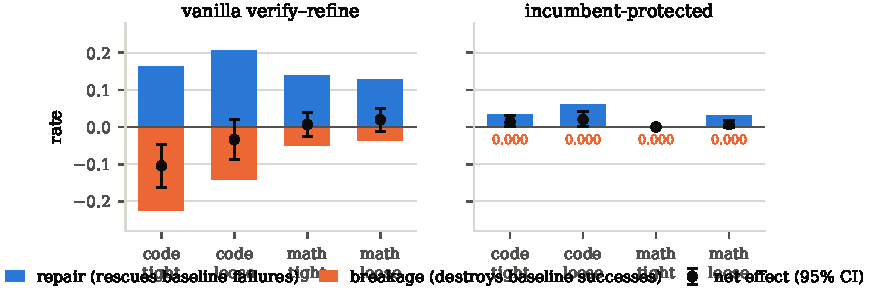
\includegraphics[width=\textwidth]{fig1_decomposition.pdf}
\caption{The same experiment, read two ways. \textbf{Left:} a standard
verify--refine workflow repairs many tasks the baseline fails (blue, above the
axis) and destroys many the baseline solves (orange, below), so the net effect
(black, 95\% CI)---the quantity the literature reports---is small and can take
either sign. \textbf{Right:} protecting the incumbent answer removes the lower
term entirely and the same machinery becomes a small, reliable gain. Frozen
test splits, three execution seeds, matched hard budgets; panels share an axis.}
\label{fig:decomposition}
\end{figure}

\section{Introduction}

A large fraction of deployed language-model systems are not single calls but
workflows: a model drafts an answer, a verifier inspects it, a refiner revises
it, and the loop repeats until something stops it. The pattern is old enough to
have a canon---self-refinement \citep{madaan2023selfrefine}, verbal
reinforcement \citep{shinn2023reflexion}, multi-agent debate
\citep{du2024debate}, self-consistency \citep{wang2023selfconsistency}---and
new enough that its value is still contested. Recent work reports that
multi-agent structure improves the compute--accuracy frontier under matched
budgets \citep{multiagent2026pareto}; other recent work argues the opposite,
that once inference compute is genuinely equalised the advantage evaporates and
reported gains reflect unaccounted computation rather than architecture. Both
camps run careful experiments. Both report a single number: the difference in
accuracy between a workflow and its baseline.

We think that number is the problem. A workflow that adds verification and
refinement does two things at once, and they point in opposite directions. It
rescues tasks the baseline would have failed---the reason anyone builds such
systems. It also damages tasks the baseline had already solved, because a
refiner asked to improve a correct answer will sometimes take it apart. Nothing
in the standard evaluation separates these. When the two are of similar
magnitude, their difference is small, unstable, and sensitive to conditions that
vary between papers: how much budget each call is allowed, how reliable the
verifier is, how strong the first draft was. A field that reports only the
difference will produce exactly the pattern we observe---careful studies that
disagree.

This paper separates them. We evaluate workflows under a reservation-based
budget ledger: before any node executes, an upper bound on its billable cost is
reserved against the remaining per-instance caps, and a node that cannot reserve
does not run. Overruns become impossible rather than merely reported, which is
what makes ``compute-matched'' mean something. Within that protocol we measure,
for every workflow and every budget, not one number but three: the repair rate
on tasks the baseline fails, the breakage rate on tasks the baseline solves, and
the net effect the two produce.

Figure~\ref{fig:decomposition} shows what this reveals. On a program-synthesis
benchmark at a \$0.25 per-task budget, a three-iteration verify--refine workflow
repairs $20.5\%$ of the baseline's failures---a real and substantial
capability---while breaking $14.0\%$ of its successes. The net is $-3.3$ points,
at $5.5\times$ the cost. Tighten the budget to \$0.10 and the same workflow
becomes significantly harmful ($-10.4$ points): with fewer affordable
iterations, repair falls and breakage rises. Withhold the verifier's signal
entirely and the effect falls to $-11.8$ points, because a refiner with nothing
to gate on rewrites correct answers along with incorrect ones. Each of these is
the movement of one term in the decomposition, produced by a controlled
manipulation of one variable.

The decomposition is not a model we fit; for binary outcomes it is an algebraic
identity, and we are explicit about that because it determines what the identity
can be used for. It cannot be validated on the data used to estimate its terms.
What it does buy is exhaustiveness---every effect a workflow has on accuracy is
repair or breakage, and there is no third channel---and, rearranged, a design
rule: refinement pays exactly when the breakage-to-repair ratio falls below
$(1-p)/p$, where $p$ is baseline accuracy. Because the ratio is a design choice,
the rule is actionable---though not in the way we first assumed. Breakage has
two paths, and gating the refiner closes only one of them: a workflow that
drafts its own answer can be wrong where the reference is right, and an
accepting verifier passes that answer through without refinement ever running.
The path closes only when the workflow's incumbent \emph{is} the reference
system's output. Under that condition, which we verify holds exactly in our
runs, breakage is $0.000$ in all six in-domain cells and is bounded by the
verifier's false-rejection rate.

A design principle derived by us from our own decomposition and then tested by
us is a route by which an intuition can be mistaken for a finding. We therefore
built a budget-safe automated search over a restricted workflow language---not
to propose a new optimiser, but to ask whether a procedure with no access to our
reasoning arrives at the same place. In the code family it does: every search
arm converges on a draft behind a verifier gate, and a single policy conditioned
on remaining budget matches per-budget static search, at both searched budgets
and at an intermediate budget it never saw, using half the search cost. The
searcher is ours, so this bounds our design bias rather than eliminating it. In the math family it does not, and we report that too.

We take the reliability of these claims as seriously as the claims themselves.
Every confirmatory hypothesis was written, committed and git-tagged before the
corresponding frozen split was executed \citep{nosek2018preregistration}, and we
report all of them as they landed: four Part-I claims supported and one refuted,
three Part-II claims not supported as stated, and a locked out-of-domain
prediction that failed---because, as \S\ref{sec:external} diagnoses, our own
out-of-domain split had been built without visible tests, so it varied domain
and verifier availability at once. An automated audit recomputes every numeric
claim in this paper from raw per-task logs.

The practical consequence is short. Structure is not free and is not uniformly
good: it has an entry fee below which it is harmful, and it requires a verifier
with signal. Where those hold, the thing worth building is not more structure
but a guarantee that structure cannot destroy what already worked.

\section{Background and related work}

\paragraph{Iterative refinement and its discontents.} Self-Refine
\citep{madaan2023selfrefine} and Reflexion \citep{shinn2023reflexion}
established the generate--critique--revise loop as a default building block, and
multi-agent debate \citep{du2024debate} and self-consistency
\citep{wang2023selfconsistency} extended the idea to populations of samples.
Sceptical results arrived quickly: \citet{huang2024selfcorrect} showed that
models cannot reliably self-correct reasoning without external feedback, and
attributed apparent gains to oracle labels leaking into the correction signal.
Our decomposition puts a quantity behind that critique. Self-correction without
external signal is exactly the regime in which $\brate$ is unconstrained, and we
measure what it costs: $-11.8$ points when the verifier is stripped of
information, with breakage rising from $0.140$ to $0.234$.

\paragraph{Automated workflow design.} A body of work searches over agent
structures rather than fixing them by hand. GPTSwarm \citep{zhuge2024gptswarm}
represents agents as optimisable graphs and jointly tunes node prompts and
edges; ADAS \citep{hu2024adas} has a meta-agent write agent code; AFlow
\citep{zhang2025aflow} searches code-level workflows with tree search;
AgentSquare \citep{shang2024agentsquare} searches a modular design space; EvoFlow
\citep{zhang2025evoflow} evolves a population of heterogeneous workflows under
cost and accuracy objectives; EvoAgentX \citep{wang2025evoagentx} packages
several such optimisers. These methods optimise \emph{within} a design space.
Our question is prior to it: what determines whether any structure in such a
space is worth its cost, and why careful comparisons disagree. Our searcher is
deliberately ordinary, because its role here is falsification rather than
performance.

\paragraph{Budget-aware inference.} \citet{li2026bavt} condition inference-tree
node selection on the remaining-resource ratio, and \citet{agentuct2026} make
workflow \emph{search} cost-aware through prefix reuse and caching. The budget
conditioning we search over acts on workflow control flow rather than on tree
node selection, and our ledger enforces caps before execution rather than
accounting for them afterwards---a distinction that matters, because a workflow
prevented from overspending behaves differently from one that overspends and is
billed for it.

\paragraph{Test-time compute allocation.} For a single model the tradeoff
between sampling more and refining longer is well studied:
\citet{snell2024scaling} show the optimal allocation depends on problem
difficulty and \citet{verification2025granularity} on verification granularity.
This is the closest antecedent to our budget floor. What it does not do, and
what we add, is separate the two directions of a workflow's effect. The
crossovers reported there are crossovers in a net quantity, and the mechanism we
identify---that structure destroys correct answers at a rate governed by
verifier specificity---is invisible to it.

\paragraph{Abstention, deferral and conservative updates.} Declining to act on
a low-confidence prediction is old: the reject option dates to
\citet{chow1970reject} and reappears as selective classification
\citep{geifman2017selective} and learning to defer
\citep{madras2018defer, mozannar2020defer}. Detector cascades
\citep{viola2001cascade} and their language-model descendants
\citep{chen2023frugalgpt} gate expensive stages on a cheap one; conservative
policy updates \citep{thomas2015safe, garcelon2020conservative} refuse changes
that cannot be shown not to regress; and regression testing
\citep{cohen1995regression} exists to stop a change from breaking what already
worked. Reference preservation as we state it is a member of this family: a
guarded fallback whose guard is a verifier and whose fallback is a reference
system's own output. What we add is not the idea of guarding but its
consequences under explicit inference budgets --- an exhaustive accounting of
where a workflow's effect comes from, a bound tying the residual to a verifier
property that can be measured beforehand, and the observation that the guard is
useless unless the guarded object is the reference's actual output.
Calibration of model self-assessment \citep{kadavath2022know} is the missing
ingredient our verifier taxonomy stands in for.

\paragraph{Evaluation.} We use MBPP+ and HumanEval+ \citep{austin2021mbpp,
chen2021humaneval} in the rigorous-test formulation of EvalPlus
\citep{liu2023evalplus}, MATH \citep{hendrycks2021math} and BIG-Bench Hard
\citep{suzgun2023bbh}; multi-fidelity screening follows successive halving
\citep{jamieson2016successive, li2018hyperband}, and intervals are stratified
paired bootstrap \citep{efron1994bootstrap} with Holm correction
\citep{holm1979}.

\section{Hard budgets and a reservation ledger}
\label{sec:setup}

\begin{figure}[t]
\centering
\begin{minipage}[b]{0.40\textwidth}
\centering
{\small\textbf{(a) reservation ledger}}\\[3pt]
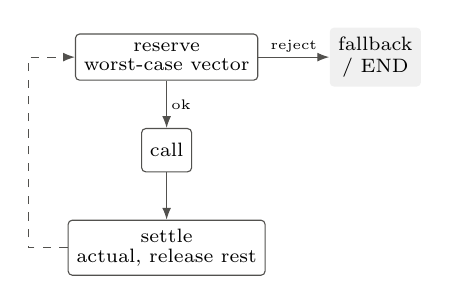
\begin{tikzpicture}[
  font=\small, node distance=4mm,
  box/.style={draw=inkgrey, rounded corners=1.5pt, minimum height=5.5mm,
              inner xsep=3pt, align=center, font=\scriptsize},
  term/.style={box, fill=black!6, draw=none},
  ar/.style={-{Latex[length=1.5mm]}, draw=inkgrey},
  lab/.style={font=\tiny, inner sep=1.5pt}]
\node[box] (res) {reserve\\[-1pt]worst-case vector};
\node[box, below=6mm of res] (call) {call};
\node[box, below=6mm of call] (set) {settle\\[-1pt]actual, release rest};
\node[term, right=9mm of res] (fb) {fallback\\/ END};
\draw[ar] (res) -- node[lab, right]{ok} (call);
\draw[ar] (call) -- (set);
\draw[ar] (res) -- node[lab, above]{reject} (fb);
\draw[ar, dashed] (set.west) -- ++(-5mm,0) |- (res.west);
\end{tikzpicture}
\end{minipage}\hfill
\begin{minipage}[b]{0.56\textwidth}
\centering
{\small\textbf{(b) identical control flow, different incumbent}}\\[3pt]
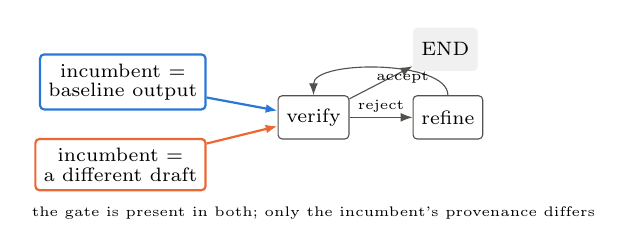
\begin{tikzpicture}[
  font=\small, node distance=4mm,
  box/.style={draw=inkgrey, rounded corners=1.5pt, minimum height=5.5mm,
              inner xsep=3pt, align=center, font=\scriptsize},
  gen/.style={box, draw=repairblue, thick},
  alt/.style={box, draw=breakorange, thick},
  term/.style={box, fill=black!6, draw=none},
  ar/.style={-{Latex[length=1.5mm]}, draw=inkgrey},
  lab/.style={font=\tiny, inner sep=1.5pt}]
\node[box] (v) {verify};
\node[box, right=8mm of v] (r) {refine};
\node[term, above right=3mm and 8mm of v] (e) {END};
\draw[ar] (v) -- node[lab, above]{reject} (r);
\draw[ar] (r.north) .. controls +(0,4.5mm) and +(0,4.5mm) .. (v.north);
\draw[ar] (v) -- node[lab, above right, pos=0.35]{accept} (e);
\node[gen, left=9mm of v, yshift=4.5mm] (i1) {incumbent $=$\\[-1pt]baseline output};
\node[alt, left=9mm of v, yshift=-6mm] (i2) {incumbent $=$\\[-1pt]a different draft};
\draw[ar, draw=repairblue, thick] (i1) -- (v);
\draw[ar, draw=breakorange, thick] (i2) -- (v);
\node[lab, below=8mm of v, align=left]
  {the gate is present in both; only the incumbent's provenance differs};
\end{tikzpicture}
\end{minipage}
\caption{\textbf{(a)} Every metered call reserves an upper bound on its billable
cost before executing; a node that cannot reserve does not run, and control
follows a fallback edge. Overruns are prevented rather than recorded.
\textbf{(b)} The two workflows we compare have \emph{identical} control flow:
both terminate on an accepted draft and refine only on rejection. What differs
is where the incumbent comes from. One reuses the reference baseline's own
output; the other independently produces a different draft (a different prompt
at a different temperature). \S\ref{sec:theory} shows this is the operative
distinction, and \S\ref{sec:limitations} records that our two arms also differ
in prompt and temperature, so the isolated contribution of each is not
established.}
\label{fig:mechanism}
\end{figure}

A deployment budget is a vector of caps on input tokens, output tokens, LLM
calls, tool calls, wall-clock seconds and dollars. We use five profiles from
\$0.02 to \$0.25 per task. Two are searched---\texttt{tight} (\$0.10, four
calls) and \texttt{loose} (\$0.25, eight calls)---and \texttt{unseen} (\$0.15)
is touched only at final evaluation, enforced by an assertion in the search path
that fails if any selection code reads it.

Before a node executes, an upper bound on its billable vector is computed and
\emph{reserved} against the remaining caps. If the reservation fails the node
does not run: control follows a fallback edge or terminates with the current
answer. After the call, actual usage is settled and the surplus released, and a
settlement exceeding its own reservation is surfaced as a defect rather than
absorbed. Concurrent calls, such as the $k$ branches of a vote, reserve their
full aggregate before any of them starts. Figure~\ref{fig:mechanism}(a) shows the discipline and
Appendix~\ref{app:safety} proves the resulting invariant and reports a $3{,}000$-workflow fuzz sweep with
zero cap violations in any dimension.

This is not only hygiene: under post-hoc accounting a workflow that overspends
is recorded as expensive, whereas under reservation it is prevented, and the
prevention becomes an observable---reserve rejections turn out to be the visible
face of the budget floor. Compute matching is enforced rather than audited.

\paragraph{Model.} All experiments use a single frozen deployment of GPT-4o
(Azure OpenAI, API version 2024-12-01-preview), fixed for the duration of the
study; the deployment identifier and version are recorded with every trace.
Unless a workflow node specifies otherwise, generation uses temperature $0.7$
and refinement $0.7$; the protected first draft uses temperature $0$. No model
is fine-tuned, and no results depend on model updates: the same deployment
served every run reported here.

\paragraph{Verifiers.} We distinguish two regimes and never conflate them. In
the code family the workflow's verifier runs the task's own visible tests:
environment feedback that is part of the task specification, with hidden
extended tests reserved for the external grader. In the math and logic families
no oracle is available to the workflow, and the verifier is a gold-free
self-consistency check that re-derives the answer independently and compares.
Gold answers never enter workflow state in any family.

\paragraph{Tasks.} Code: MBPP+, split 120/40/150 for search, selection and
confirmation, with HumanEval+ held out. Math: MATH levels 4--5 over four
subjects, split 120/40/150, with two further subjects held out. Logic:
BIG-Bench Hard, 120 tasks, reserved for \S\ref{sec:external} and used nowhere
else. Splits were generated once with a fixed seed, hashed, and never
regenerated. All final numbers use three execution seeds, seed-averaged per
task, with stratified paired bootstrap intervals over $10{,}000$ resamples.

\section{The repair--breakage decomposition}
\label{sec:theory}

Let $B$ be a baseline and $W$ a workflow evaluated on the same tasks under the
same budget. Write $p=\Pr[B\text{ correct}]$ and
\begin{equation}
\rrate = \Pr[W \text{ correct} \mid B \text{ incorrect}], \qquad
\brate = \Pr[W \text{ incorrect} \mid B \text{ correct}],
\end{equation}
so that the net change in accuracy is
\begin{equation}
\Delta \;=\; \Pr[W] - \Pr[B] \;=\; (1-p)\,\rrate \;-\; p\,\brate.
\label{eq:identity}
\end{equation}

Equation~\ref{eq:identity} holds exactly, by the law of total probability, for
binary per-task outcomes. We state this plainly because it determines what the
equation is good for. It cannot be ``validated'' by estimating $\rrate$ and
$\brate$ on a dataset and checking that it reproduces $\Delta$ there; that check
is tautological, and we do not present one. What it establishes is that the
decomposition is \emph{exhaustive}: every effect a workflow has on accuracy is
repair or breakage. A literature that reports only $\Delta$ is reporting a
difference of two quantities each of which can be an order of magnitude larger
than the difference itself.

Rearranged, \eqref{eq:identity} gives a condition for when refinement is worth
running:
\begin{equation}
\frac{\brate}{\rrate} \;<\; \frac{1-p}{p}.
\label{eq:rule}
\end{equation}
Two regimes follow. With an oracle verifier that never rejects a correct answer,
$\brate \to 0$ and refinement cannot hurt. With a verifier carrying no
information every answer is flagged, $\brate$ rises to the unconditional rate at
which revision damages correct answers, and \eqref{eq:rule} fails whenever the
baseline is strong---which, for a competent model on a standard benchmark, it
is. The threshold is punishing: $p=0.73$ demands $\brate/\rrate < 0.38$ and
$p=0.92$ demands $\brate/\rrate < 0.09$.

The rule is actionable because its left-hand side is a design choice, though not
the one we first supposed. Consider a workflow that emits an incumbent $I$,
accepts it when a verifier does, and otherwise refines it into $J$. Writing $R$
for rejection, breakage decomposes into two paths:
\begin{equation}
\brate = \underbrace{\Pr(\neg R,\, I \text{ wrong} \mid B\text{ correct})}
         _{\text{a wrong incumbent the verifier accepted}}
       + \underbrace{\Pr(R,\, J \text{ wrong} \mid B\text{ correct})}
         _{\text{refinement failed after a rejection}} .
\label{eq:twoterm}
\end{equation}
The first term is the one that matters and the one the gate does not touch: if
the workflow's incumbent is some answer of its own, it can be wrong on a task
the reference solves, and an accepting verifier then hands that wrong answer
straight through. No refinement is involved. Gating the refiner cannot remove
this path, because the path never reaches the refiner.

It vanishes under one condition. If $I = B$ --- the workflow's incumbent is the
reference system's actual output, not merely an answer produced under the same
configuration --- then $B$ correct implies $I$ correct, the first term is
identically zero, and
\begin{equation}
\brate = \Pr(R,\, J\text{ wrong} \mid B\text{ correct})
       \;\le\; \Pr(R \mid B\text{ correct}).
\label{eq:bound}
\end{equation}
We call this \emph{reference preservation}. It is a condition on provenance
rather than a control-flow feature: a workflow does not regress against a
reference unless the verifier first falsely rejects that reference's own
answer. Equality in \eqref{eq:bound} holds only if every false rejection ends
in a wrong answer.

The distinction matters because $I=B$ is not implied by configuring the
incumbent's generator identically to the baseline. Nominally deterministic
decoding does not guarantee byte-identical outputs across calls. In our runs
the condition does hold exactly --- among executions where the verifier
accepted, the workflow's output is byte-identical to the baseline's in
$402/402$ code and $396/396$ math cases --- but it holds because both calls
resolve to the same response-cache entry, not because determinism was
established. A deployment that wants the guarantee should reuse the reference's
stored output rather than regenerate it.

Unlike \eqref{eq:identity}, \eqref{eq:bound} is falsifiable on data: its
left-hand side is measured on the workflow and its right-hand side on the
verifier alone, so a single condition with breakage above its own
false-rejection rate would refute it. Figure~\ref{fig:bound} puts it to that
test in all ten conditions we ran, spanning verifiers that almost never reject a
correct draft and verifiers that reject every draft. It holds in all ten, and is
close to tight in the middle of that range. The practical reading is that the
false-rejection rate is measurable before deployment, from the verifier alone,
and it caps how much a gated workflow can cost you. Sections~\ref{sec:parti} and
\ref{sec:external} test whether this works, where it fails, and whether the
parameters transfer. They do not transfer for unconstrained workflows; they do
for constrained ones, which is a claim about our construction rather than a law.

\begin{figure}[t]
\centering
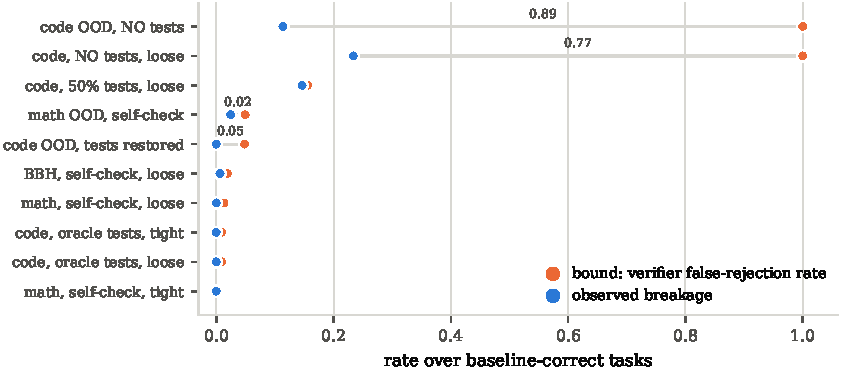
\includegraphics[width=\textwidth]{fig_bound.pdf}
\caption{The bound \eqref{eq:bound} against measurement, in every condition we
ran. Its left-hand side is a property of the verifier alone and can be measured
without executing the workflow: a gated workflow that exits after its verifier
accepted the draft leaves a different trace from one that proceeds to refine, so
the false-rejection rate is recoverable from logs already collected. Observed
breakage falls below the bound in all ten conditions, across the full range from
a verifier that almost never rejects a correct draft ($0.009$) to one that
rejects every draft because it has no information ($1.000$). The bound is nearly
tight where the verifier is moderately noisy---breakage $0.146$ against a bound
of $0.156$ under $50\%$ test masking---and loose where it is uninformative,
because refinement sometimes recovers an answer it has just discarded. Rates are
over baseline-correct tasks.}
\label{fig:bound}
\end{figure}

\section{Confirmatory experiments}
\label{sec:parti}

Five claims were written, committed and tagged (\texttt{prereg-freeze-partI})
before any frozen test split was executed. We report all five.

\begin{table}[t]
\caption{Frozen test splits, 150 tasks per family, three execution seeds.
Baselines are the strongest single-call structure per family (direct prompting
for code, chain-of-thought for math). \emph{Vanilla} is
generate$\to$verify$\to$refine with up to three iterations; \emph{protected} is
the same loop with a temperature-zero incumbent replaced only on verifier
rejection. Intervals are stratified paired bootstrap 95\% CIs. The
\texttt{unseen} (\$0.15) budget behaves between the two shown and is reported in
Appendix~\ref{app:floor}.}
\label{tab:parti}
\centering
\small
\begin{tabular}{lllrrrr}
\toprule
Family & Budget & Workflow & $\Delta$ (95\% CI) & repair & breakage & \$/task \\
\midrule
code & tight  & vanilla   & $-0.104$ $[-0.162,-0.047]$ & $0.162$ & $0.224$ & $0.0062$ \\
code & tight  & protected & $+0.013$ $[+0.002,+0.031]$ & $0.034$ & $\mathbf{0.000}$ & $0.0022$ \\
code & loose  & vanilla   & $-0.033$ $[-0.087,+0.020]$ & $0.205$ & $0.140$ & $0.0090$ \\
code & loose  & protected & $+0.020$ $[+0.002,+0.042]$ & $0.060$ & $\mathbf{0.000}$ & $0.0025$ \\
\midrule
math & tight  & vanilla   & $+0.007$ $[-0.027,+0.040]$ & $0.140$ & $0.050$ & $0.0076$ \\
math & tight  & protected & $+0.000$ $[+0.000,+0.000]$ & $0.000$ & $\mathbf{0.000}$ & $0.0075$ \\
math & loose  & vanilla   & $+0.020$ $[-0.011,+0.051]$ & $0.129$ & $0.037$ & $0.0153$ \\
math & loose  & protected & $+0.007$ $[-0.002,+0.018]$ & $0.032$ & $\mathbf{0.000}$ & $0.0153$ \\
\bottomrule
\end{tabular}
\end{table}

\paragraph{The net effect is zero and the terms are not (C1, supported).} At
\texttt{loose}, vanilla verify--refine differs from its baseline by $-0.033$
$[-0.087,+0.020]$ in code and $+0.020$ $[-0.011,+0.051]$ in math, at $5.5\times$
and $2.2\times$ the cost. Neither interval excludes zero: the workflow buys
nothing measurable at several times the price. The decomposition shows what is
happening underneath---in code it repairs a fifth of the baseline's failures and
destroys a seventh of its successes.

\paragraph{Structure has an entry fee (C2, supported).} At \texttt{tight}, code
vanilla is $-0.104$ $[-0.162,-0.047]$. Moving from \texttt{loose} to
\texttt{tight}, repair falls from $0.205$ to $0.162$ while breakage rises from
$0.140$ to $0.224$: with fewer affordable iterations the loop is likelier to
leave a task mid-revision, having already discarded a working answer. Both terms move together (Figure~\ref{fig:floor}, Appendix~\ref{app:floor}). The
mechanism is visible in the ledger: 35 of 150 tasks could not fund a planned
refinement call, and at the point of refusal the ledger shows three or four
calls used against a cap of four, with dollars at $\$0.008$ against a cap of
$\$0.10$. The binding constraints are the call and output-token caps, not
dollars. Because our profiles move several caps together, this establishes a
crossover across composite profiles and not an entry fee in a named resource;
a single-dimension scan is required and we do not have one.

\paragraph{Breakage is controlled by the verifier (C3, supported).} Masking
visible tests at $1.0 \to 0.5 \to 0.0$ moves the code/\texttt{loose} effect
monotonically: $-0.033$, $-0.033$, $-0.118$ $[-0.178,-0.058]$, with breakage
climbing from $0.140$ to $0.234$. Because masking changes only the verifier this
is a causal manipulation of the $\brate$ term (Figure~\ref{fig:signal},
Appendix~\ref{app:floor}, left panel).
It also supplies a mechanism for the sceptical literature: refinement without
external signal does not merely fail to help, it destroys correct work.

\paragraph{C4, \textcolor{red}{unsupported as preregistered}.} We registered
the claim that adding incumbent protection---understood as a structural change,
gating the refiner on the verifier---would eliminate breakage. An audit of our
own implementation, carried out after the confirmatory runs, showed that both
compared workflows already had that gate: their control flow is identical edge
for edge. The comparison therefore never manipulated the variable the claim was
about, and we mark C4 unsupported as stated rather than restate it to fit what
the comparison did manipulate.

\paragraph{What the comparison did manipulate, and a post-hoc proposition.} The
arms differed in where the incumbent came from (Figure~\ref{fig:mechanism}(b)).
In the reference-preserving arm
the first call is configured exactly as the baseline's and, because both resolve
to the same response-cache entry, returns byte-identical text: among executions
where the verifier accepted, $402/402$ code and $396/396$ math outputs are
identical to the baseline's. Under that condition \eqref{eq:twoterm} gives a
proposition we did not preregister and state here as \emph{post hoc}, motivated
by the audit: if a workflow emits the reference system's own output as its
incumbent, emits it unchanged on acceptance, and can reach a different answer
only after rejection, then acceptance-path regression is impossible and
$\brate \le \Pr(R \mid B\text{ correct})$. Consistent with it, no breakage event
occurs in any of the six reference-preserving cells; at code/\texttt{loose} a
task-clustered one-sided $95\%$ upper bound over $107$ baseline-correct tasks is
$0.027$, against a measured false-rejection rate of $0.009$. Two cautions belong
with this: $I=B$ is a property of our \emph{implementation}, delivered by a
shared cache entry rather than by decoding determinism; and a proposition
formulated after seeing the data cannot be confirmed by it
(\S\ref{sec:limitations}).

\paragraph{Repair is not bounded by verifier type (C5,
\textcolor{red}{refuted}).} We predicted that oracle-verified repair would
strictly exceed non-oracle repair, with the math interval containing zero.
Observed: code repair $0.060$ $[0.000,0.137]$, math repair $0.032$
$[0.000,0.075]$. The intervals overlap substantially. Gold-free self-consistency
checking produces real repair, and we make no claim about verifier-type-bounded
repair beyond these intervals.

\paragraph{A check on our own design space.} Reference preservation was derived
by us and tested by us, so we asked whether a search procedure given a design
space we specified in advance, and no access to the derivation, selects the same
construction. It does select low-temperature drafts behind a verifier gate, but
we do not read this as rediscovery: every candidate in the space carries the
gate, and the space does not contain the choice that \eqref{eq:twoterm} says
matters---whether to reuse a reference system's stored output. Of five
preregistered claims, three fail, including cost reduction and non-inferiority
in the math family; what survives is that at an unseen \$0.15 budget the code
policy is indistinguishable from its preregistered static control
(Figure~\ref{fig:protocolA}, Appendix~\ref{app:searchdetail}) at half the
search cost. Appendix~\ref{app:searchdetail} gives the protocol and every
per-claim result.

\section{External validity}
\label{sec:external}

\paragraph{A locked prediction that failed.} Before computing any out-of-domain
effect we committed (tag \texttt{ood-predictions-locked}) predictions for
HumanEval+ and held-out math subjects, transferring $\rrate$ and $\brate$ from
the in-domain frozen split. The prediction failed: mean absolute error $0.061$,
sign agreement $6/8$, and the structural breakage bound violated in code at
$0.125$ and $0.114$.

\paragraph{The confound was ours.} Our out-of-domain code split had been
constructed with empty visible tests, so its verifier ran in the no-signal
regime while the transferred parameters came from the oracle regime: the test
varied domain \emph{and} verifier availability simultaneously. Substituting
matched no-signal parameters does not rescue it either (errors $0.09$--$0.15$),
so the quantitative transfer claim fails on its own terms and we do not make it.
We then built the condition we should have built in the first place: visible
tests recovered from HumanEval+ docstring examples ($68/100$ tasks), differing
from in-domain only in domain. Breakage returns to $0.000$
(Table~\ref{tab:regimes}), and the transferred prediction is accurate for
protected workflows (errors $0.002$ and $0.000$) while remaining badly wrong for
vanilla ones ($0.169$, $0.108$)---the constrained-versus-unconstrained asymmetry
of \S\ref{sec:theory}.

\begin{table}[t]
\caption{Breakage of the reference-preserving workflow across verifier regimes
and domains. Consistent with \eqref{eq:bound}, what varies is the verifier
rather than the domain: the one condition whose verifier has no signal is an
order of magnitude worse than the rest, and restoring signal on the same tasks
restores the result.}
\label{tab:regimes}
\centering
\small
\begin{tabular}{llrr}
\toprule
Condition & Verifier & breakage & $\Delta$ (95\% CI) \\
\midrule
in-domain code (MBPP+) & oracle tests & $0.000$ & $+0.020$ $[+0.002,+0.042]$ \\
in-domain math (MATH) & non-oracle check & $0.000$ & $+0.007$ $[-0.002,+0.018]$ \\
out-of-domain math (held-out subjects) & non-oracle check & $0.025$ & $-0.003$ $[-0.027,+0.017]$ \\
out-of-domain code (HumanEval+) & \emph{none} & $0.114$ & $-0.087$ $[-0.140,-0.033]$ \\
out-of-domain code, signal restored & recovered tests & $0.000$ & $+0.005$ $[+0.000,+0.015]$ \\
new domain (BIG-Bench Hard) & non-oracle check & $0.006$ & $+0.025$ $[+0.003,+0.050]$ \\
\bottomrule
\end{tabular}
\end{table}

\paragraph{A prospective test in a third domain.} Everything above is
retrospective. To test the account prospectively we chose a domain no part of
this project had touched---BIG-Bench Hard logical deduction, shuffled-object
tracking and date understanding \citep{suzgun2023bbh}, 120 multiple-choice tasks
with exact-match grading and a gold-free verifier---committed our predictions
(\texttt{prospective-locked}), and only then ran anything. They were structural,
since the parameters had already been shown not to transfer: breakage
$\le 0.02$ under reference preservation, materially higher without it, and a
non-negative effect. The first and third hold in all four cells ($0.000$,
$0.006$, $0.000$, $0.003$; effects $\ge 0$), in a demanding regime where the
baseline is right $92$--$94\%$ of the time so \eqref{eq:rule} demands
$\brate/\rrate < 0.09$. The second does not: at \texttt{loose} the unprotected
variant also breaks only $0.006$. Breakage requires that refinement be
\emph{able} to destroy a correct answer, and with single-label answers and a
$94\%$ baseline there is little to destroy; at \texttt{tight}, where refinement
acts under pressure, the gap reappears ($0.026$ against $0.000$). Reference
preservation is insurance, and its premium is visible only where the risk is.

\section{Limitations}
\label{sec:limitations}

\paragraph{One model.} Every number comes from GPT-4o. Both $p$ and $\rrate$
depend on model quality and $\brate$ plausibly does too; nothing here establishes
that the tradeoff transfers across model scales, and our own tests show the
parameters are unstable even across domains for unconstrained workflows. A
weaker model has a lower $p$, which by \eqref{eq:rule} loosens the threshold and
should make structure easier to justify --- a prediction we have not tested.

\paragraph{The identity is not a forecast.} \eqref{eq:identity} is exact for
binary outcomes; its content is exhaustiveness plus the rule \eqref{eq:rule},
and it makes no prediction falsifiable on the data used to estimate its terms.
The genuine transfer tests are those of \S\ref{sec:external}, one of which failed.

\paragraph{The reference-preservation proposition is untested.} It was
formulated after auditing our implementation and is not established by the runs
that motivated it. Testing it needs arms differing only in incumbent
provenance---one reusing a stored reference output by explicit assignment rather
than by cache coincidence, one regenerating under the same policy, one drafting
under a different policy---with cross-arm caching disabled so the first two are
distinguishable. We have not run it.

\paragraph{Two measurement defects in the released data.} A token estimator
that under-counted punctuation-dense prompts caused $4.7\%$ of frozen-test
executions to be scored as failures, unevenly across arms, and our math
grader's symbolic-equivalence branch never executed, misgrading $2.6\%$ of
math answers. Both are fixed; both left traces in the released data. We
re-graded every stored response at no additional inference cost, which moved
the math baseline from $0.700$ to $0.733$ and cost two math sub-claims their
significance, and we recompute every headline contrast on the defect-free
subset. The breakage results are unaffected and the harm effects grow slightly.
Appendices~\ref{app:sensitivity} and \ref{app:regrade} give both analyses in
full; both gradings are retained in the released data.

\paragraph{Further limits, stated in full in Appendix~\ref{app:scope}.} We
cannot explain with data why the searched policy is better at math/\texttt{loose}
and worse at math/\texttt{tight}; our one-shot selection uses a 40-task split
whose variance swamps the gaps between candidates; results about ``structure''
are results about our restricted language; and our three-way verifier taxonomy
stands in for a continuum of sensitivity and specificity.

\section{Conclusion}

Whether agent workflow structure helps has no budget-free answer, and reporting
a net effect conceals why. Structure repairs and structure breaks; under matched
hard budgets the two are of comparable size, so their difference is small and
reads differently depending on where in the budget range one measures. Once
separated, \eqref{eq:twoterm} shows the design question is not whether to gate
the refiner---gating leaves untouched the path where a verifier accepts a
workflow's own wrong draft---but whose answer the workflow is holding when the
verifier speaks. Hand it the reference system's output and that path closes,
leaving a residual bounded by a quantity anyone can measure from the verifier
alone. What remains open is the comparison this construction invites: whether,
at genuinely matched spend, any of this beats sampling more and picking well.

\subsubsection*{Reproducibility statement}

All splits are hashed and frozen. Every confirmatory claim was git-tagged before
the corresponding split was executed (\texttt{prereg-freeze-partI},
\texttt{prereg-freeze-partII}, \texttt{ood-predictions-locked},
\texttt{prospective-locked}). The anonymised repository contains the workflow
language and its validator, the reservation ledger with its fuzz harness, every
search registry with parent and mutation lineage, all raw per-task traces under
both gradings, the preregistration with its append-only deviation log including
the refuted claims, and a single command that recomputes every table and figure
in this paper from raw logs and exits non-zero on any disagreement.

\subsubsection*{AI use statement}

Language models were used as coding assistants during implementation, and are the
subject of study. All experimental design decisions, preregistered hypotheses,
analyses and claims are the authors' own, and every reported number is recomputed
from raw logs by the audit script in the repository.

\bibliography{refs}
\bibliographystyle{iclr2027_conference}

\appendix
\section{Workflow language}
\label{app:dsl}

A workflow is a JSON graph validated statically before any spend. Node
whitelist: \texttt{generate}, \texttt{refine}, \texttt{vote} ($k\le 5$),
\texttt{verify}, \texttt{decompose}, \texttt{aggregate}, \texttt{branch},
\texttt{END}. Structural constraints: at most $8$ nodes; at most $2$ loops, each
with \texttt{max\_iter} $\le 3$; every node must reach \texttt{END} via non-loop
edges, checked by reachability. Edge conditions come from a fixed grammar:
\texttt{always}, \texttt{verify\_passed}, \texttt{verify\_failed},
\texttt{budget\_below:$q$}, \texttt{budget\_above:$q$}, with $q\in(0,1)$ read
against the ledger's most-binding remaining fraction. The meta-agent emits JSON
patches only; no model-generated text is executed as program logic. Candidate
solutions to code tasks are executed, but only inside a network-isolated
subprocess with a 5\,s CPU limit and a 4\,GB address-space limit. Invalid
candidates are rejected at zero API cost, and we report the invalid rate
alongside search cost rather than hiding it.

\section{Budget safety}
\label{app:safety}

\begin{proposition}
Fix a task, a budget profile $C$, and any workflow expressible in the language.
If (i) every metered call is preceded by a successful reservation of an upper
bound on its billable vector, (ii) concurrent calls reserve their full aggregate
before any of them starts, and (iii) every settlement reports actual usage no
greater than its reservation, then cumulative usage never exceeds $C$ in any
countable dimension.
\end{proposition}

\begin{proof}[Proof sketch]
Induct on the number of settled calls, with invariant
$\textit{used} + \textit{reserved} \le C$ componentwise. It holds initially.
A reservation is admitted only if the invariant survives adding its vector to
\textit{reserved}; a settlement moves a quantity no larger than the reservation
from \textit{reserved} to \textit{used} and releases the remainder, which cannot
increase the sum. Rejected reservations leave the state unchanged and divert
control flow, so no unreserved call occurs.
\end{proof}

Wall-clock time is not reservable, since its consumption is not known in
advance; it is metered continuously and enforced by admission checks plus
per-call deadlines. Provider-side cancellation latency is reported separately
from policy-attributable overruns. A fuzz sweep of $3{,}000$ randomly generated
legal workflows against randomly drawn budget profiles, with a mocked model,
produced zero cap violations in any dimension.

Assumption (iii) is an assumption about the \emph{estimator}, and ours was
initially wrong: a characters-per-token heuristic under-counted
punctuation-dense code prompts by roughly $55\%$, so some settlements exceeded
their own reservations. The implementation surfaces these as defects rather than
absorbing them, which is how we found them.
Appendix~\ref{app:sensitivity} quantifies the residual effect on the frozen test
results, which were collected before the estimator was replaced with an exact
tokeniser count plus a $5\%$ margin.

\section{Failure taxonomy}
\label{app:failures}

Categories were fixed before inspection. Counts are over all failures in the
frozen test split at seed 0, pooled across structures and budgets.

\begin{center}
\small
\begin{tabular}{lrl}
\toprule
Category & share & example \\
\midrule
first draft wrong, no refinement triggered & $28.4\%$ & \texttt{direct}, mbpp\_103 \\
premature budget exhaustion (reserve rejected) & $26.3\%$ & protected math, algebra\_1071 \\
verifier passed a wrong answer & $19.8\%$ & protected code, mbpp\_113 \\
ledger defect (settle overrun; see \ref{app:sensitivity}) & $18.4\%$ & protected code, mbpp\_578 \\
refined but still wrong (signal insufficient) & $7.1\%$ & protected code, mbpp\_160 \\
\bottomrule
\end{tabular}
\end{center}

The third row is the mechanism behind $\brate$: a verifier that accepts an
incorrect answer cannot trigger the repair that would fix it, and one that
rejects a correct answer invites the breakage that destroys it.

\section{Budget profiles and verifier signal}
\label{app:floor}

\begin{figure}[t]
\centering
\begin{minipage}[t]{0.485\textwidth}
\centering
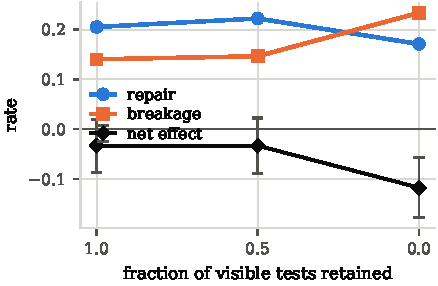
\includegraphics[width=\textwidth]{fig4_dose_response.pdf}
\end{minipage}\hfill
\begin{minipage}[t]{0.485\textwidth}
\centering
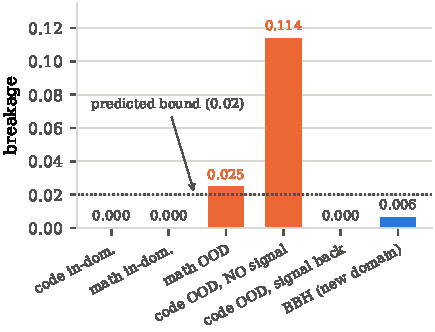
\includegraphics[width=\textwidth]{fig5_regimes.pdf}
\end{minipage}
\caption{\textbf{Left:} withholding the verifier's signal is a causal
manipulation of the breakage term. As visible tests are removed, breakage rises
and repair falls, and the net effect drops to $-0.118$ $[-0.178,-0.058]$.
\textbf{Right:} breakage of the incumbent-protecting construction across every
condition we measured, including a third domain whose prediction was locked
before execution. It stays at or near the predicted bound wherever the verifier
carries signal and jumps to $0.114$ in the single condition with none;
restoring signal on the \emph{same} tasks restores the guarantee.}
\label{fig:signal}
\end{figure}

\begin{figure}[t]
\centering
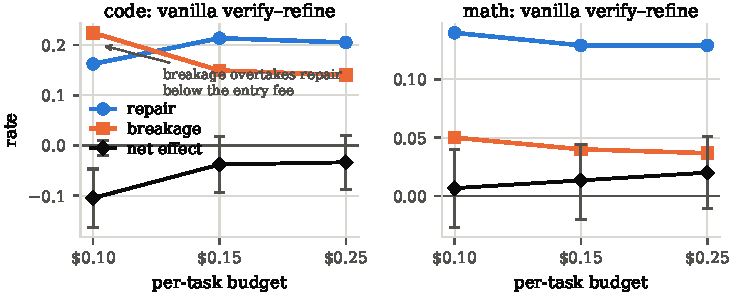
\includegraphics[width=\textwidth]{fig3_budget_floor.pdf}
\caption{Both terms move together as the budget profile tightens: the workflow
affords fewer refinement iterations, repair falls, breakage rises, and in the
code family they cross where the net effect turns significantly negative.
Profiles are named rather than dollar-valued because the dollar cap is not the
binding constraint --- realized spend is \$0.002--\$0.015 against caps of
\$0.10--\$0.25, and admission failures are caused by the call and output-token
caps. \texttt{tight} $=$ (4 calls, 8k in, 2k out, \$0.10);
\texttt{unseen} $=$ (6, 12k, 3k, \$0.15); \texttt{loose} $=$ (8, 16k, 4k,
\$0.25). Which dimension binds is not identified by these composite profiles;
see \S\ref{sec:limitations}. Frozen test splits, 95\% CIs on the net effect.}
\label{fig:floor}
\end{figure}

\section{Sensitivity to the ledger defect}
\label{app:sensitivity}

$4.7\%$ of frozen-test executions ($466/9{,}900$) terminated with a settlement
overrun, unevenly across arms (protected $6.5\%$, vanilla $4.5\%$, baseline
$3.6\%$), and were scored as failures. We recompute every headline contrast on
the subset of tasks where \emph{neither} arm hit the defect in \emph{any} seed.

\begin{center}
\small
\begin{tabular}{lrrr}
\toprule
Contrast & all tasks & defect-free subset & $n$ \\
\midrule
C1 code loose, vanilla $-$ direct & $-0.033$ $[-0.087,+0.020]$ & $-0.046$ $[-0.096,+0.005]$ & 146 \\
C2 code tight, vanilla $-$ direct & $-0.104$ $[-0.162,-0.047]$ & $-0.115$ $[-0.173,-0.056]$ & 148 \\
C3 code loose, no signal & $-0.118$ $[-0.178,-0.058]$ & $-0.132$ $[-0.192,-0.074]$ & 144 \\
C4 code tight, protected & $+0.013$ $[+0.002,+0.031]$ & $+0.014$ $[+0.002,+0.032]$ & 147 \\
C4 code loose, protected & $+0.020$ $[+0.002,+0.042]$ & $+0.018$ $[+0.002,+0.041]$ & 145 \\
C4 code unseen, protected & $+0.020$ $[+0.002,+0.042]$ & $+0.021$ $[+0.002,+0.043]$ & 146 \\
\bottomrule
\end{tabular}
\end{center}

Breakage of the protected construction is $0.000$ under both views in every
cell, so C4's structural claim is unaffected, and the C1--C3 harm effects become
slightly \emph{larger} on the defect-free subset, so those conclusions are not
artifacts of the defect.

\section{Math re-grading}
\label{app:regrade}

Our math grader compares a boxed answer by string match, then numerically, then
by symbolic equivalence. The third stage never fired: the symbolic library was
absent from the environment that produced the frozen runs, and the import sits
inside an exception handler. Because every model response is stored, re-grading
required no additional inference. $623$ of $24{,}334$ stored math answers
($2.6\%$) changed grade, almost all of them formatting variants of the same
value. The math baseline moved from $0.700$ to $0.733$. Two math sub-claims lost
significance (protected at \texttt{unseen} and at \texttt{loose}); no verdict
changed, and breakage remained $0.000$ in every in-domain protected cell. All
numbers in this paper use the corrected grading; the original field is preserved
on disk.

\section{Automated search: protocol and per-claim results}
\label{app:searchdetail}

Incumbent protection was derived by us, from our own decomposition, and tested
by us. We therefore asked whether a search procedure, given a design space we
specified in advance and no access to that derivation, selects the same
construction. It is a bound on our design bias, not an independent replication:
the node whitelist, the edge grammar and the objective are ours.

The searcher evolves workflows in the restricted language of
Appendix~\ref{app:dsl} under multi-fidelity racing
\citep{jamieson2016successive}, scoring candidates jointly at both searched
budgets. Its budget-contingent and static arms differ only in whether edges may
read remaining budget. At full fidelity on the search split every arm selected
the same shape---a low-temperature draft, a verifier gate, refinement only on
rejection. We no longer read this as the search having rediscovered our
principle. Every candidate in the space carries the verifier gate, so selecting
it is not evidence about the mechanism of \eqref{eq:twoterm}; and the space does
not contain the choice that matters, namely whether to reuse a reference
system's stored output as the incumbent. What the search does show is a
preference for low-temperature drafts, which is consistent with, but does not
isolate, reference preservation. Of five preregistered confirmatory claims
(\texttt{prereg-freeze-partII}), three fail: non-inferiority holds in code at
both budgets and at math/\texttt{loose} but not at math/\texttt{tight}; the cost
reduction reaches $10.5\%$ against a $20\%$ threshold, and in math the searched
policy is $191\%$ \emph{more} expensive in exchange for $+0.049$ accuracy, a
Pareto trade rather than a saving; and only $3$ of $12$ selected policies retain
the gated shape, because the preregistered one-shot selection uses a 40-task
validation split whose variance swamps the $1$--$2$ point gaps between
candidates. What survives is narrow: at an unseen \$0.15 budget the code policy
is indistinguishable from the preregistered static control ($-0.001$
$[-0.013,+0.010]$) at half the search cost, and a search over our design space
does select the gated pattern there. Appendix~\ref{app:searchdetail} gives the
full protocol and per-claim results.



Incumbent protection was derived by us, from our own decomposition, and tested
by us. We therefore built a searcher to check whether a procedure with no access to
that reasoning selects the same construction from a space we specified in
advance.

Candidates are workflows in a restricted language: at most eight nodes, at most
two loops of at most three iterations, a fixed node whitelist, no
model-generated executable code, and static validation before any spend
(Appendix~\ref{app:dsl}). Search is evolutionary with multi-fidelity racing over
nested task subsets \citep{jamieson2016successive}, evaluating every candidate
jointly at both searched budgets and ranking by a score that averages per-budget
accuracy with the worst budget, so a candidate cannot win by specialising. The
budget-contingent arm and the static control differ only in whether edges may
condition on remaining budget; over 200 sampled workflows the static arm never
emitted a budget predicate. Protocol A gives the static control a full search
budget \emph{per} budget tier, twice what the budget-contingent arm receives.

\paragraph{Selection variance in Part II.} Our preregistered rule selects a
policy once on a 40-task validation split, which cannot resolve the $1$--$2$
point gaps between candidates---hence shape convergence is universal in the
search-split analysis but $3/12$ among selected policies. A larger validation
split is the fix; we did not retrofit it after the freeze.

\paragraph{Restricted design space, coarse verifier taxonomy.} Results about
``structure'' are results about a space of at most eight nodes and two loops with
a fixed whitelist, and we treat verifiers as oracle, non-oracle-with-signal or
no-signal, whereas real verifiers vary continuously in sensitivity and
specificity. \eqref{eq:identity} folds both into $\rrate$ and $\brate$;
separating them would give a sharper rule and is the obvious next step.

\section{Search details}
\label{app:search}

\begin{figure}[t]
\centering
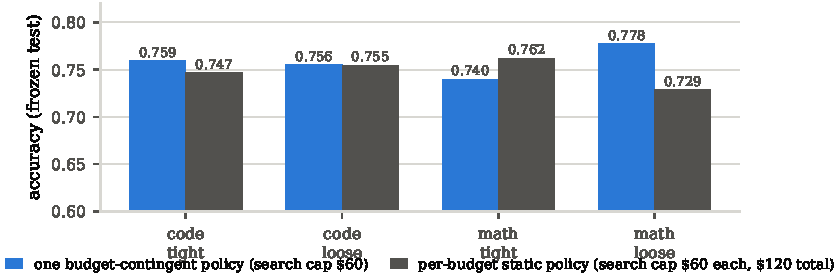
\includegraphics[width=\textwidth]{fig6_protocolA.pdf}
\caption{Protocol A on the frozen test split: one budget-contingent policy
against the static policy searched specifically for each budget, which received
twice the total search budget. We deliberately do not plot the two search
procedures' internal scores against each other---the budget-contingent score is
a cross-budget minimum and the static score is a single-budget value, so one
axis would compare incomparable quantities. Deployment accuracy at a given
budget is comparable, and is what is shown. Code figures average three search
seeds.}
\label{fig:protocolA}
\end{figure}


\paragraph{A note on the racing rule.} Our first implementation compared a
candidate's lower confidence bound against the incumbent's with a fixed slack of
$0.10$. The Hoeffding half-width \citep{hoeffding1963} differs by $0.107$ between
the $n{=}24$ and $n{=}64$ rungs, so promotion from the cheapest rung was
arithmetically impossible and almost no candidate ever left it. Whenever rung
sizes differ, racing must compare a candidate's \emph{upper} bound against the
incumbent's lower bound; a fixed slack cannot substitute for the difference in
interval widths. No result reported in this paper comes from runs made before
this was corrected.

Fidelity rungs are nested prefixes of the search split: $24$, $64$ and $120$
tasks, with $1$, $1$ and $2$ execution seeds. Racing eliminates a candidate only
when its Hoeffding upper bound falls below the incumbent's lower bound at the
same or a higher rung. Selection and archive ranking use a fidelity-comparable
mean-based score; the conservative bound is used only for the racing rule.

\begin{center}
\small
\begin{tabular}{lrrrr}
\toprule
Run (code, search seed 0) & candidates & spend & rung distribution & archive \\
\midrule
budget-contingent & 33 & \$63.0 & 9/5/19 & 11 \\
static @ tight & 76 & \$60.7 & 35/5/36 & 38 \\
static @ loose & 30 & \$61.6 & 5/5/20 & 8 \\
\bottomrule
\end{tabular}
\end{center}

\section{Scope of the design space and verifier taxonomy}
\label{app:scope}

\paragraph{No mechanism for the math search boundary.} The budget-contingent
policy is better at math/\texttt{loose} and worse at math/\texttt{tight}, and we
cannot explain this with data. It would be easy to present it as a boundary
predicted by \eqref{eq:rule}; the measured ratio sits essentially on the
threshold, so the rule is silent there and does not predict harm. We do not
claim it does.

\section{What response caching did and did not affect}
\label{app:cacheaudit}

Caching was enabled for the structure-library runs (Appendix~\ref{app:cost}),
which is how the reference-preserving arm came to hold a byte-identical copy of
the baseline's output. A reader is entitled to ask what else it touched. We
audited three questions against the implementation and the stored logs.

\paragraph{Were the three execution seeds collapsed into one?} No. The cache key
is a hash over the deployment name, the message list, and a parameter dictionary
that includes the execution seed, so runs at different seeds cannot share an
entry. Empirically, across the frozen test split, $102$--$150$ of $150$ tasks
per cell produce different outputs across the three seeds. The seed-averaging
and the intervals built on it therefore rest on genuinely repeated executions.

\paragraph{Did a cache hit escape the budget ledger?} No. The reservation is
taken \emph{before} the cache is consulted, and a hit is settled against that
reservation with the stored token counts, so a cached call consumes call count,
tokens, and dollars exactly as a fresh one does and can be refused by the same
admission check. The budget-floor result of \S\ref{sec:parti} is consequently
not an artifact of caching; what caching changes is the invoice and the wall
clock, neither of which carries a claim in this paper.

\paragraph{What caching did change.} Two things. It made the invoice roughly a
quarter of the logical figure. And, because the baseline's call and the
reference-preserving arm's first call are configured identically at a given
seed, it made them resolve to one entry --- which is why $\Pr[I{=}B]=1$ holds
exactly rather than approximately. That is a coupling between arms, and we
treat it as part of the treatment definition rather than as an incidental
detail: the comparison is between an arm holding the reference's own output and
an arm holding a different draft, and caching is the mechanism that made the
first arm's incumbent exact. A design that wants the property rather than
inheriting it should assign the stored reference output directly, as
\S\ref{sec:limitations} notes.

\section{Cost accounting}
\label{app:cost}

We separate two cost figures that are easy to conflate.

\textbf{Per-task deployment cost} --- every dollar figure in the tables --- is a
\emph{logical} cost: what the workflow would cost with no response caching. This
is the quantity a deployment faces, because a deployed system meets new tasks and
cannot serve them from a cache of its own past answers. Reporting cache-assisted
prices in those tables would understate deployment cost substantially.

\textbf{Study cost} is the actual invoice, which is much smaller. Response
caching was enabled for the structure-library runs, including those on the
frozen test split, so identical calls across arms resolved to a single API
request. The ledger charges a cached call exactly as it charges a fresh one,
which is why no reported quantity changes; but it also means the two figures
diverge by the cache hit rate. Summed over every experiment reported here the
logical figure is \$1{,}317.74, against \$2{,}000 as the ledger's
circuit-breaker cap, while the billed figure is roughly \$300 --- consistent
with $77{,}942$ unique cached responses serving $194{,}318$ task executions.
Only the searched-policy evaluations of Appendix~\ref{app:searchdetail} ran with
caching disabled.

Caching also has a methodological consequence used elsewhere in this paper: it
is why identically configured calls returned identical text, and therefore why
$\Pr[I{=}B]=1$ held exactly rather than approximately (\S\ref{sec:theory}).

\section{Preregistration and outcomes}
\label{app:prereg}

The repository contains the preregistration with an append-only deviation log.
Claims were committed and git-tagged before the corresponding frozen split was
executed. Outcomes as recorded: Part I C1--C3 supported, C4 unsupported as
preregistered (the comparison did not manipulate the registered variable) and
C5 refuted; Part II
P1--P3 not supported as stated, P4 weaker than on the search split, P5 reported;
the locked out-of-domain transfer prediction failed; the prospective predictions
PV1 and PV3 held and PV2 did not.

\end{document}
